\documentclass[crop,tikz]{standalone}                 
\usepackage{physics}
\makeatletter                                                                                        

\newcommand{\sq}[1]{\frac{1}{\sqrt{#1}}}

\begin{document}

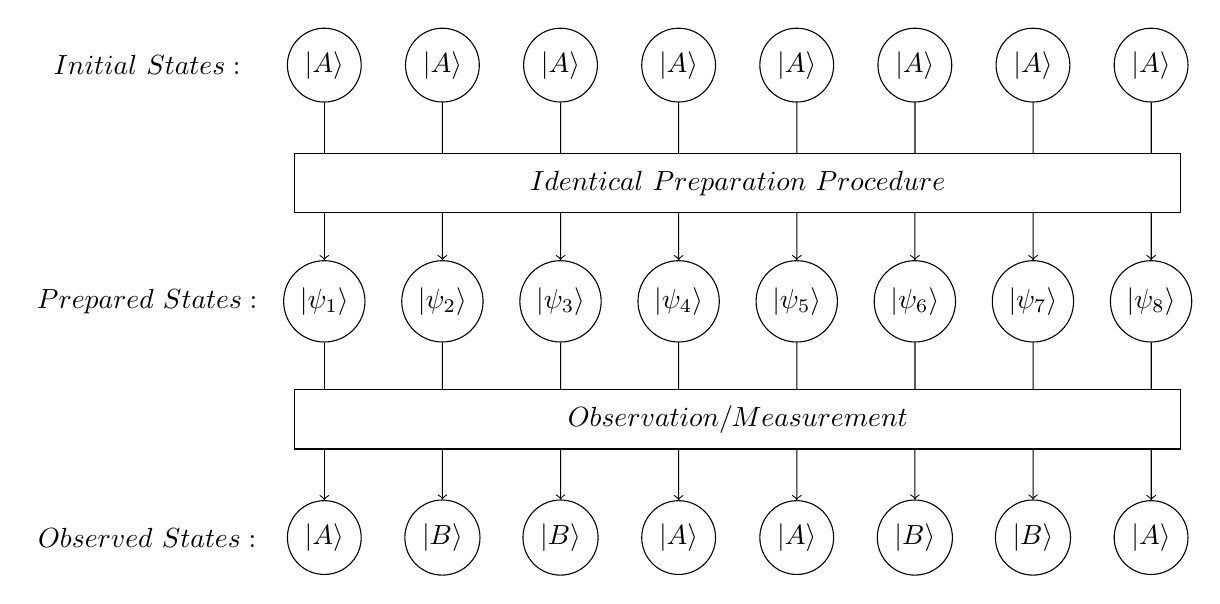
\begin{tikzpicture}[scale=1.5]                                                                          
\
%\draw [dotted] (0,0) grid (9, 4);

% system: initial states
\foreach \x in {0,1,...,7}
{
\node (x\x) [draw, circle] at (\x, 4) {$\ket{A}$};
}

% system: prepared states
\foreach \y/\k in {0/1,1/2,2/3,3/4,4/5,5/6,6/7,7/8}
{
\node (y\y) [draw, circle] at (\y, 2) {$\ket{\psi_{\k}}$};
}

% system: observed states
\node (z0) [draw, circle] at (0, 0) {$\ket{A}$};
\node (z1) [draw, circle] at (1, 0) {$\ket{B}$};
\node (z2) [draw, circle] at (2, 0) {$\ket{B}$};
\node (z3) [draw, circle] at (3, 0) {$\ket{A}$};
\node (z4) [draw, circle] at (4, 0) {$\ket{A}$};
\node (z5) [draw, circle] at (5, 0) {$\ket{B}$};
\node (z6) [draw, circle] at (6, 0) {$\ket{B}$};
\node (z7) [draw, circle] at (7, 0) {$\ket{A}$};

% arrows
\foreach \w in {0,...,7}
{
\draw [->] (x\w) -- (y\w);
\draw [->] (y\w) -- (z\w);
}

% labels
\node (init)  at (-1.50, 4.00) {$Initial   \text{ } States:$};
\node (prep) at (-1.50, 2.00) {$Prepared  \text{ } States:$};
\node (Obs)  at (-1.50, 0.00) {$Observed  \text{ } States:$};

% prepare and measure
\draw [fill=white] (-0.25, 2.75) rectangle (7.25 ,3.25) 
                                 node[pos=0.5] {$Identical\text{ } Preparation\text{ }Procedure$};
\draw [fill=white] (-0.25, 0.75) rectangle (7.25 ,1.25) 
                                 node[pos=0.5] {$Observation/Measurement$};

\end{tikzpicture}                                                                                    

\end{document}
